\documentclass[a4paper,11pt]{report}

\usepackage[T1]{fontenc}
\usepackage[utf8]{inputenc}
\usepackage[italian]{babel}

\usepackage{chemmacros}
\usepackage{mathtools}
\usepackage{graphicx}
\usepackage{amsfonts}
\usepackage{amsthm}
\usepackage{amsmath}
\usepackage{amssymb}
\usepackage{fancyhdr}
\usepackage{float}
\usepackage{geometry}
\geometry{a4paper, top=2.5cm, bottom=2cm, left=2cm, right=2cm}
\usepackage{hyperref}
\hypersetup{
	colorlinks=true,
	linkcolor=black,
	filecolor=blue,
	citecolor = black,      
	urlcolor=cyan,
}

\newtheorem*{es}{Esempio}

\begin{document}
	\date{}
	\author{Marco Militello}
	\title{Chimica}
	\maketitle
	\tableofcontents
	\newpage
	
\chapter{Introduzione}
La chimica è lo studio della materia, delle sue proprietà, delle trasformazioni subite dalla materia e dell'energia associata a queste trasformazioni
\begin{description}
	\item[Materia] Tutto ciò che ha una massa e un volume
	\item[Composizione] I tipi e le quantità di sostanze più semplici che costituiscono la materia
	\item[Proprietà] Le caratteristiche che conferiscono a ciascuna sostanza la sua identità esclusiva 
\end{description}
\section{Stati aggregazione della materia}
\begin{itemize}
	\item Un \emph{solido} ha forma e volumi fissi. I solidi possono essere duri, teneri, rigidi o flessibili
	\item Un \emph{liquido} si adatta alla forma del recipiente, ma un volume fisso. Un liquido forma una superficie
	\item Un \emph{gas} si adatta alla forma del recipiente e lo riempie completamente, perciò non forma una superficie
\end{itemize}
\section{Proprietà della materia}
\subsection*{Proprietà fisiche}
Le proprietà che una sostanza presenta di per sè senza trasformasi in, o interagire con, un'altra sostanza
\begin{itemize}
	\item[-] colore, temperatura di fusione, densità
\end{itemize}
\subsection*{Proprietà chimiche} 
Le proprietà che una sostanza presenta quando si trasforma in, o interagisce con, un'alra sostanza
\begin{itemize}
	\item[-] infiammabilità, corrosività
\end{itemize}
\section{Composizione della materia}
\subsection*{Sostanze pure}
Una sostanza che ha proprietà e composizione proprie, che non dipendono dal campione \newline
Le sostanze pure possono essere sostanze elementari (\emph{elementi}) o \emph{composti}. I composti possono essere trasformati in sostanze elementari tramite trasformazioni chimiche
\subsection*{Miscele}
Una sostanza che ha una composizione variabile, le cui proprietà dipendono dal campione analizzato \newline
Le miscele possono essere separate nelle sostanze costituenti mediante metodi fisici
\begin{figure}[H]
	\centering
	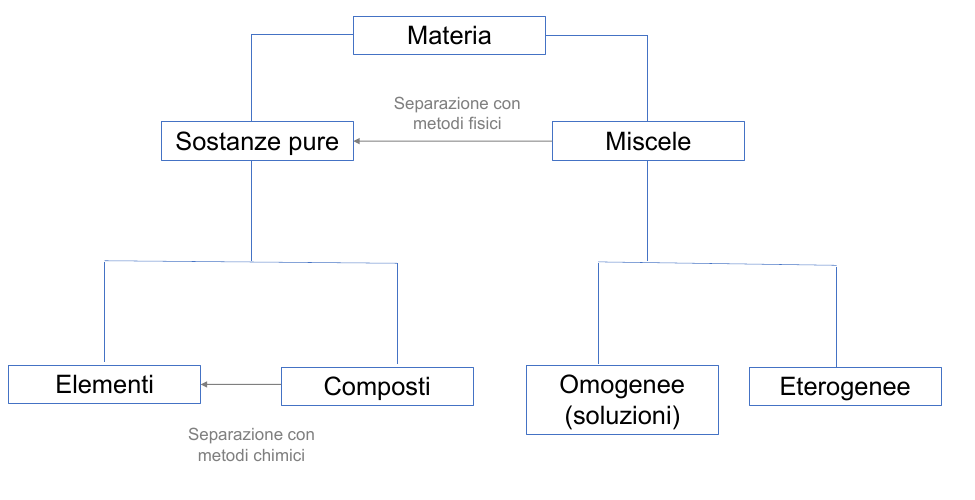
\includegraphics[width=\textwidth,height=\textheight,keepaspectratio]{immagini/grafico1}
	\label{fig:grafico1}
\end{figure}
\chapter{Teoria atomica}
\section{Teoria atomica di Dalton}
\begin{enumerate}
	\item Tutta la materia è costituita da atomi, piccole particelle indivisibili di un elemento che non possono essere nè create, nè distrutte
	\item Gli atomi di un elemento non possono essere convertiti in atomi di un altro elemento
	\item Gli atomi di un elemento sono identici nella massa e nelle altre proprietà e sono diversi dagli atomi di qualsiasi altro elemento \label{3}
	\item I composti sono formati dalla combinazione di uno specifico rapporto di atomi differenti
\end{enumerate}
\noindent La teoria di Dalton spiega le leggi delle combinazioni chimiche
\begin{itemize}
	\item Legge della composizione definita \hfil\\
	Indipendentemente dalla sua fonte, un particolare composto chimico è costituito dagli stessi elementi negli stessi rapporti in massa
	\item Legge della conservazione della massa \hfill\\
	In base al postulato \hyperref[3]{3} della legge di Dalton gli atomi, e quindi la loro massa, vengono conservati nelle reazioni chimiche
\end{itemize}
\section*{Scoperta delle particelle sub-atomiche: raggi catodici}
\begin{itemize}
	\item Il raggio devia in presenza di un campo elettrico o magnetico $\Rightarrow$ Consiste in particelle cariche di cui si determina il rapporto carica/massa
	\item In presenza di un campo elettrico esterno il raggio devia verso la rica positiva $\Rightarrow$ Consiste in particelle negative
	\item Il raggio è identico per ogni catodo $\Rightarrow$ Le particelle fanno parte di tutta la materia
\end{itemize}
\subsection*{Esperimento di Millikan}
\begin{figure}[H]
	\centering
	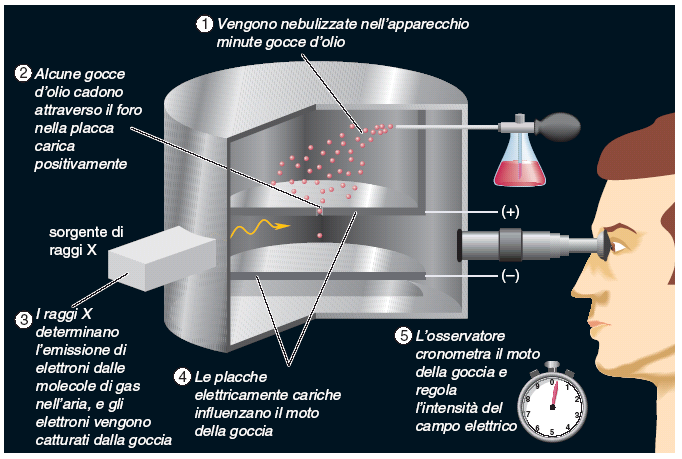
\includegraphics[width=0.5\textwidth,height=\textheight,keepaspectratio]{immagini/Millikan}
	\label{fig:millikan}
\end{figure}
\[\text{massa elettrone} = \left(\frac{massa}{carica}\right)carica = 9.109 \times 10^{-28}g  \]
\begin{figure}[H]
	\centering
	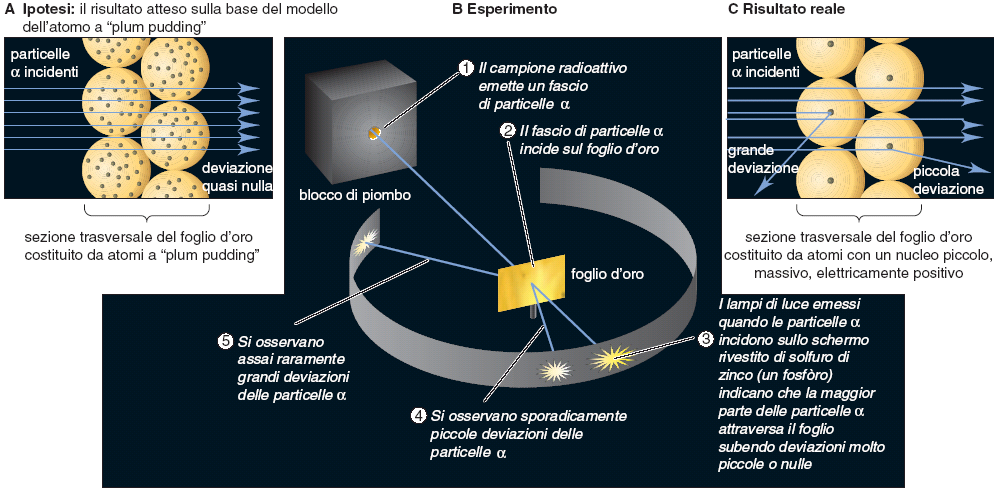
\includegraphics[width=\textwidth,height=\textheight,keepaspectratio]{immagini/atomo}
	\caption{}
	\label{fig:atomo}
\end{figure}
\begin{figure}[H]
	\centering
	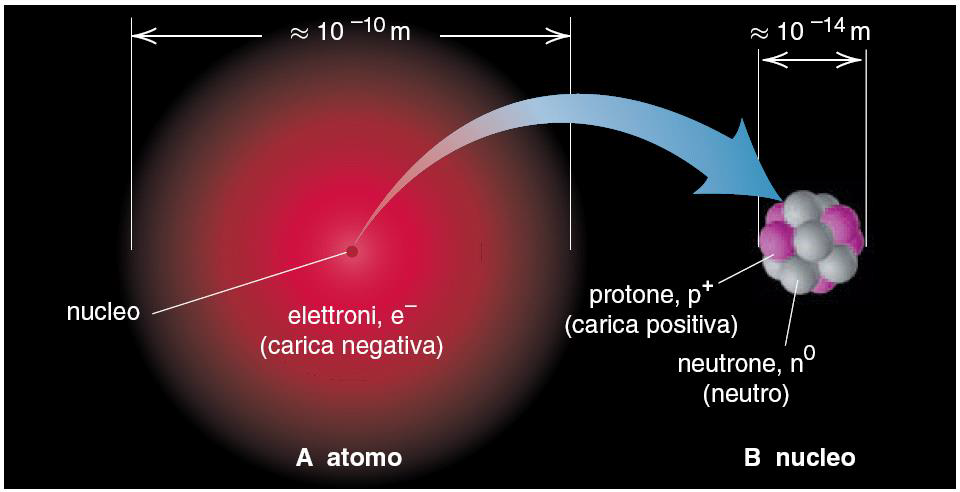
\includegraphics[width=0.5\linewidth, height=\textheight,keepaspectratio]{immagini/atomo1}
	\label{fig:atomo1}
\end{figure}
\begin{itemize}
	\item [A.] Una nuvola di elettroni carichi negativamente, in modo rapido, occupa pressochè tutto il volume atomico e circonda il minuscolo nucleo centrale
	\item [B.] Il nucleo contiene pressochè tutta la massa dell'atomo ed è costituito da protoni carichi positivamente e neutroni elettricamente neutri
\end{itemize}

\section{Simbolo atomico, numero atomico e numero di massa}

\begin{figure}[H]
	\centering
	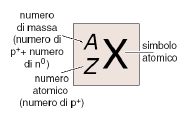
\includegraphics[width=0.2\linewidth, height=\textheight,keepaspectratio]{immagini/numero.png}
	\label{fig:numero}
\end{figure}

\begin{center}
\begin{tabular}{|c|c|}
	\hline
	X & simbolo atomico dell'elemento \\
	\hline
	Z & numero atomico (numero di protoni nel nucleo) \\
	\hline
	A & numero di massa	\\
	\hline
\end{tabular}
\end{center}

\[A = Z+N\]

\subsection*{Isotopi}

Gli isotopi sono atomi di un elemento con lo stesso numero di protoni, ma con diverso numero di neutroni; gli isotopi hanno lo stesso numero atomico, ma diverso numero di massa

\subsection*{Teoria atomica moderna}

\begin{enumerate}
	\item Tualla la materia è costituita da atomi. L'atomo è la particella più piccola che identifica univocamente un elemento 
 \item Gli atomi di un elemento non possono trasformarsi negli atomi di un altro elemento in una trasformazione chimica. Elementi possono convertiti in atri elementi solo in una reazione nucleare 
 \item Tutti gli atomi di un elemento hanno lo stesso numero di protoni e elettroni che determina il comportamento chimico dell'elemento. Gli isotopi di un elemento differiscono nel numero di neutroni, dunque nel numero di massa. Un campione di elemento viene considerato come se tutti i suoi atomi avessero una massa mediante
 \item i composti sono formati dalla combinazione chimica di due o più elementi in rapporti specifici
\end{enumerate}

\subsection*{Tecniche di separazione fondamentali}

\begin{description}
	\item[Filtrazione:] separa i componenti di una miscela sulla base di differenze tra le dimensioni delle particelle. La filtrazione viene usata spesso per separare un solido da un liquido 
 \item[Cristallizzazione:] la separazione è basata sulle differenze di solubilità dei componenti di una miscela 
 \item[Distillazione:] separa i componenti sulla base di differenze di volubilità 
 \item[Estrazione:] la separazione è basata sulle differenze di solubilità in diversi solventi
 \item[Cromatografia:] la separazione è basata sulle differenze di solubilità in una fase stazionaria     
\end{description}

\section{Atomi e molecole}
Una molecola è un'unità strutturale indipendente costituita da uno o più atomi, tenuto insieme da legami chimici (legami covalenti). Una molecola è la più piccola particella di una sostanza che ne mantenga la composizione e le proprietà chimiche. Le molecole sono le unità fondamnetali dei composti molecolari

\subsection*{Formule chimiche}
In una formula chimica, i simboli degli elementi e i pedici numerici indicano la specie e il numero di ciascun atomo presente nella più piccola unità della sostanza. Esistono più tipi di formule chimiche di una composto

\begin{description}
	\item[Formula empirica:] mostra il numero relativo di atomi in ciascun elemento nel composto. \'E il tipo più semplice di formula chimica
 \item[Formula molecolare:] mostra il numero reale di atomi di ciascun elemento in una molecola di composto
 \item[Formula di struttura:] mostra il numero di atomi e i legami tra di essi, cioè le posizioni reciproche e le connessione degli atomi nella molecola    
\end{description}

\begin{description}
	\item[Ione:] un singolo atomo (ione monoatomico) o un gruppo di atomi (ione poliatomico) legati mediante legami covalenti che ha una carica netta 
 \item[Catione:] ione di carica positiva (\# protoni > \# elettroni)
 \item[Anione:] ione di carica negativa (\# elettroni > \# protoni)  
\end{description}

\noindent I composti ionici sono costituiti da ioni, che sono l'unità fondamentale

\chapter{Stechiometria}
\subsection*{Studio delle relazioni di massa in chimica}

Masse atomiche: le masse relative gli atomi dei diversi elementi si esprimono secondo le loro masse atomiche 
\[u = \frac{1}{12}m(\ch{^{12}C})\]
Nella tavola periodica è riportata la massa atomica media pesata per l'abbondanza isotopica \newline
Massa molecolare: la massa molecolare si ottiene sommando le masse atomiche secondo la formula chimica \newline
Per i composti ionici si parla di massa forumla perchè i composti ionici non sono costituiti da molecole 

\subsection*{Mole}
Le trasformazioni chimiche avvengono in seguito a reazioni tra atomi, molecole o ioni; è quindi fondamentale conoscere il numero di atomi presenti nella massa di sostanza sottoposta a reazione. \newline
La \textbf{mole} (mol) è la quantità di sostanza che contiene tante entità elementari quante sono gli atomi in 12g di \ch{^{12}C}; il termine entità si riferisce ad atomi, ioni, molecole, unità di formula, elettroni - ogni tipo di particelle \newline
Una mole contiene $6.022\times 10^{23}$ entità; si chiama numero di Avogadro e si indica con $N_A$

\subsection*{Massa molare}
La massa molare M di una sostanza è numericamente uguale alla massa di una mole di sue entità espressa in grammi; per gli elementi monoatomici, la massa molare, espressa in grammi per mole, è numericamente uguale alla massa atomica, espressa in unità di massa atomica. La massa atomica si legge sulla tavola periodica \newline
Per gli elementi molari e per i composti, è necessario conoscere la formula per determinare la massa molare 
\noindent m: massa(g) \quad n: numero di moli (mol) \quad M: massa molare $\left(\frac{g}{mol}\right)$ \quad $N_A$: numero di Avogadro \newline 
N: numero di entità

\begin{align*}
	n = \frac{m}{M} \qquad  m &= nM \\
	n = \frac{N}{N_A} \qquad  N &= nN_A
\end{align*}

\noindent Per un elemento \qquad  Massa elemento $\xrightarrow[]{M}$ Quantità di massa $\xrightarrow[]{\text{numero di Avogadro}}$ atomi elementi \newline
Per un composto \qquad Massa composto $\xrightarrow[]{M}$ Quantità di composto $\xrightarrow[]{\text{numero di Avogadro}}$ Molecole di composto 

\subsection*{Percentuale in massa della formula chimica}
\[\% A = \frac{m_A}{m_{totale}} \times 100\]
La percentuale in massa può anche essere utilizzata per calcolare la massa di un particolare elemento in una data massa di composto

\subsection*{Formule empiriche}
La formula empirica è la formula più semplice di un composto che sia in accordo con le analisi elementari. Mostra i numeri di moli interi più piccoli e dà il numero di atomi relatico di ogni elemento

\subsection*{Formula molecolare}
La formula molecolare mostra il numero reale di atomi di ciascun elemento in una molecola di composto \newline
La formula molecolare è un multiplo secondo un numero intero della formula empirica 

\section{Equazioni chimiche}
Un'equazione chimica è un enunciato in formula che esprime le identitò e quantità delle sostanze che partecipano a una trassformazione chimica o fisica \newline

Una freccia indica la trasformazione dei reagenti nei prodotti; i reagenti si scrivono a sinistra, mentre i prodotti a destra \newline
L'equazione deve essere bilanciata: lo stesso numero e tipo di atomi deve comparire nei due membri dell'equazione 

\subsection*{Bilanciare un'equazione chimica}
\begin{itemize}
	\item traduzione dell'enunciato
 \item bilanciare gli atomi usando i coefficienti stechiometrici: le formule non possono essere modificate
 \item correggere i coefficienti se necessario
 \item verificare che l'equazione sia bilanciata
 \item specificare lo stato fisico
\end{itemize}

\subsection*{Calcoli stechiometrici}
I coefficienti in un'equazione chimica bilanciata rappresentano i numeri relativi di particelle di reagenti e prodotti e i relativi numeri di moli. Poichè le moli sono correlate alla massa, l'equazione può essere utilizzata per calcolare masse di reagenti e/o prodotti coinvolti in una data reazione; i rapporti molari derivanti dall'equazione bilanciata rappresentano i fattori di conversione 

\subsection*{Reazioni in sequenza}
Le reazioni avvengono spesso in sequenza: il prodotto di una reazione diventa il reagente della successiva; la reazione complessiva è la somma delle varie reazioni. Ogni sostanza che si forma in una reazione ed è utilizzata in quella successiva può essere eliminata

\subsection*{Reagenti limitanti}
Un reagente può limitare la quantità di prodotto che si formare. Il reagente limitante sarà completamente consumato nella reazione, mentre parte del reagente che non è limitante (eccesso) rimarrà inalterata alla fine della reazione 

\subsection*{Resa}
\begin{description}
	\item[Resa teorica:] quantità di prodotto calcolata utilizzando i rapporti molari dell'equazione bilanciata 
 \item[Resa effettiva:] quantitò di prodotto ottenuta nella realtà
\end{description}

\[\text{Resa percentuale } = \frac{\text{resa effettiva}}{\text{resa teorica}} \times 100 \]

\section{Percentuale in massa dalla formula chimica}
\begin{equation*}
	\% A = \frac{m_A}{m_{tot}} \times 100
\end{equation*}
La percentuale in massa può anche essere utilizzata per calcolare la massa di un particolare elemento in una data massa di composto

\section{Formule empiriche e molecolari}
La formula empirica è la formula più semplice di un composto che sia in accordo con le analisi elementari. Mostra i numeri di moli interi più piccoli e dà il numero di atomi relativo di ogni elemento 

\begin{es}
	La formula empirica del perossido di idrogeno è HO
\end{es}

\noindent La formula molecolare mostra il numero reale di atomi di ciascun elemento in una molecola di composto

\begin{es}
	La formula molecolare del perossido di idrogeno è $H_2O_2$
\end{es}

\subsection*{Determinare la formula molecolare}
La formula molecolare mostra il numero reale di atomi di ciascun elemento in 1 mole di composto. La formula molecolare è un multiplo intero della formula empirica
\begin{equation*}
	\frac{\text{massa molecolare (g/mol)}}{\text{massa della formula empirica (g/mol)}} = \text{multiplo intero}
\end{equation*}
Si possono avere diversi composti che hanno la stessa formula molecolare, ma con proprietà
\begin{es}
	Etanolo e Dimetiletere
\end{es}

\section{Equazioni chimiche}
Un'equazione chimica è un enunciato in formule che esprime le identità e le quantità delle sostanze che partecipano a una trasformazione chimica o fisica

\begin{es}
	\begin{equation*}
		H_2(g) + F_2(g) \longrightarrow 2HF(g)
	\end{equation*}
\end{es}

\noindent Una freccia indica la trasformazione dei reagenti nei prodotti; i reagenti si scrivono a sinistra, i prodotti si scrivono a destra \newline
L'equazione deve essere bilanciata: lo stesso numero e tipo di atomi deve comparire nei due membri dell'equazione \newline
Per bilanciare un'equazione chimica bisogna seguire i seguenti passaggi
\begin{enumerate}
	\item traduzione dell'enunciato
	\item bilanciare gli atomi usando i coefficienti stechiometrici: le formule non possono essere modificate
	\item correggere i coefficienti se necessario
	\item vericare che l'equazione sia bilanciata
	\item specificare lo stato fisico: solido (s), liquido puro (l), sostanza gassosa (g), ione o molecola in soluzione acquosa (aq)
\end{enumerate}
I coefficienti in un'equazione chimica bilanciata rappresentano i numeri relativi di particelle di reagenti e prodotti e i relativi numeri di moli; poicheè le moli sono correlata alla massa, l'equazione può essere utilizzata per calcolare masse di reagenti e/o prodotti coinvolti in una data reazione. I rapporti molari derivanti dall'equazione bilanciata rappresentano i fattori di conversione

\subsection*{Reazioni in sequenza}
Le reazioni avvengono spesso in sequenza: il prodotto di una reazione diventa il reagente della successiva. la reazione complessiva (reazione netta) è la somma delle varie reazioni. Ogni sostanza che si forma in una reazione ed è utilizzata in quella successiva può essere eliminata

\chapter{Teoria quantistica e spettri atomici}

Gli atomi sono costituiti da nuclei estremamente piccoli come sede della quasi totalità della massa dell'atomo e di tutte le cariche positive; gli elettroni nel loro moto intorno al nucleo contribuiscono a dare volume all'atomo

\section{Debolezze modello planetario atomo}

Un nucleo e un elettrone si attraggono reciprocamente e quindi, affichè rimangano separati, l'energia cinetica degli elettroni deve bilanciare l'energia potenziale di attrazione nucleo-elettrone. Le leggi della fisica classica avevano stabilito che una particella negativa in moto in una traiettoria curva attorno ad una particella posiviva doveva emettere radiazione e quindi perdere energia: quindi l'elettrone dovrebbe cadere sul nucleo con una traiettoria a spirale. Inoltre con questo modello non è possibile trattare gli atomi multi-elettronici (repulsione elettronica) e la formazione reversibile di legami di chimici tra atomi \newline
Per spiegare il comportamento degli elettroni nell'atomo dobbiamo abbandonare i concettti della fisica classica e introdurre i concetti della fisica quantistica. La comprensione del comportamento degli elettroni dell'atomo è derivato dall'analisi della luce emessa o assorbita delle sostanze

\section{Luce}

La luce visibile è un tipo di radiazione elettromagnetica, detta anche energia radiante. Le proprietà ondulatorie delle radiazioni elettromagnetiche sono descritte da tre variabili
\begin{itemize}
	\item frequenza (n): cicli al secondo
	\item lunghezza d'onda (l): distanza percorsa dall'onda in un ciclo
	\item ampiezza: l'altezza di massimo e la profondità di un minimo
\end{itemize}
La velocità della radiazione elettromagnetica è una costante
\begin{equation*}
	c = \nu \lambda = 3.00 \times 10^8 \frac{m}{s}
\end{equation*}
Fenomeno importante che riguarda le onde è la formazione di figure di interferenza

\section{Radiazione di corpo nero e quantizzazione dell'energia}

Un corpo solido emette luce visibile quando viene riscaldato a circa 1000 K. Questa radiazione è chiamata radiazione di corpo nero. \newline
Il colore e l'intensità della luce variano al variare della temperatura. Il colore è correlato alla lunghezza d'onda e alla frequenza, mentre la temperatura è correlata all'energia. L'energia è perciò correlata alla lunghezza d'onda e alla frequenza:
\begin{equation*}
	E = nh\nu
\end{equation*}
dove n è un numero positivo e h è la costante di Planck che vale $6.626 \times 10^{-34} Js$

\section{Quantizzazione dell'energia}

Ogni oggetto (inclusi gli atomi) può emettere o assorbire determinate quantità di energia. L'energia è quantizzata: esiste solo in quantità fisse invece di essere continua. Ogni quantità fissa di energia è detta quanto. Un atomo può cambiare il suo stato energetico solo mediante l'assorbimento o l'emissione di quanti di energia
\begin{equation*}
	\Delta E = nh \nu
\end{equation*}
con $h\nu$ energia di quanto \newline
Noi non ci accorgiamo che l'enrgia è quantizzata perchè la costante di Planck è molto piccola e quindi la quantizzazione dell'energia non impatta il mondo macroscopico, ma diventa rilevante a livello atomico

\section{Effetto fotoelettrico e fotoni}

La luce incidente che impatta su una superficie metallica causa l'emissione di elettroni. 
Una frequanza minima della luce, diversa per ogni metallo è necessaria per avere emissione di elettroni.
Per spiegare l'effetto fotoelettrico, Einstein assunse che la radiazione elettromagnetica si comportasse come un fascio di pacchetti di energia, che chiamò fotoni.
\begin{equation*}
	E = h\nu \qquad \text{energia fotone}
\end{equation*}
Gli elettroni vengono emessi dal metallo solo se i fotoni hanno energia ( e quindi frequenza) sufficiente a vincere le forza attrattice che tengono l'elettrone al metallo

\section{Spettro a righe dell'idrogeno}
Analisi spettrale di una radiazione policromatica (contenente diverse lunghezze d'onda)

\subsection*{Tre serie di righe spettrali per l'atomo di idrogeno}

Equazione di Rydberg
\begin{equation*}
	\frac{1}{\lambda} = R_H \left(\frac{1}{n^2_1}-\frac{1}{n^2_2}\right)
\end{equation*}
con $R_H$ costante di Rydberg che vale $1.096776 \times 10^7 m^{-1}$; per la serie visibile $n_1=2$ e $n_2 = 3,4,5,\dots$ 

\subsection*{Modello di Bohr atomo di idrogeno}

Il modello atomico di Bohr è basato su 3 postulati:
\begin{enumerate}
	\item L'atomi di idrogeno ha soltanto certi livelli energetici permessi (stati stazionari) a ognuno dei quali è associata un'orbita circolare fissa dell'elettrone attorno al nucleo
	\item L'atomo non irraggia energia mentre è in uno dei suoi stati stazionari
	\item L'atomo compie una transizione in un altro stato stazionario soltanto assorbendo o emettendo un fotone la cui energia è uguale alla differenza di energia dei due stati ($\Delta E = h\nu$)
\end{enumerate}
Quando l'elettrone dell'atomo di idrogeno H si trova nella prima orbita, l'atomo è nello stato fondamentale, il livello energetico più basso. 
Quando l'elettrone è in una qualsiasi orbita con n>1 l'atomo è in uno stato eccitato

\section{Dualismo onda particella di materia e energia}

Materia ed energia sono forme alternative della stessa entità
\begin{equation*}
	E = mc^2
\end{equation*}
Tutta la materia mostra proprietà sia delle particelle che delle onde. Gli elettroni si muovono di moto ondulatorio e possono avere soltanto certi valori permessi di frequenze ed enegie. 
Anchela materia ha natura ondulatoria, e la lunghezza d'onda di de Broglie per una qualsiasi particella è data da 
\begin{equation*}
	\lambda = \frac{h}{mu}
\end{equation*}
con m massa e u velocità

\section{Principio di indeterminazione di Heisenberg}

Non è possibile conoscere simultaneamente posizione esatta e quantità di moto esatta di una particella
\begin{equation*}
	\Delta x \cdot m \Delta u \ge \frac{h}{4\pi}
\end{equation*}
Maggiore è l'accuratezza con cui conosciamo la velocità, minore è l'accuratezza con cui conosciamo la posizione e viceversa

\section{Il modello quantomeccanico dell'atomo}

La meteria-onda associata all'elettrone si muove nello spazio attorno al nucleo da cui è continuamente influenzata. L'elettrone è descritto da una funzione d'onda. 
L'equazione d'onda di Schrodinger ci permette di calcolare i livelli energetici permessi per gli elettroni in un atomo. 
Il quadrato della funzione d'onda dà la densità di probabilità, una misura della probabilità di trovare un elettrone con una particolare energia in una particolare regione dell'atomo

\section{Numeri quantici e orbitali}

La soluzione dell'equazione di Schrodinger per l'atomo di idrogeno dà luogo a un set di funzioni d'onda chiamate orbitali. 
Un orbitale atomico è specificato da 3 numeri quantici
\begin{itemize}
	\item Il numero quantico principale (n) è un intero positivo. Il valore di n indica la dimensione relativa dell'orbitale e, conseguentemente, la sua distanza relativa dal nucleo
	\item Il numero quantico del momento angolare (l) è un numero intero compreso tra 0 e (n-1). Il valore di l indica la forma dell'orbitale
	\item Il numero quantico magnetico ($m_l$) è un numero intero compreso tra -l e +l. Il valore di m indica l'orientazione dell'orbitale
\end{itemize}

\subsection*{Numeri quantici per gli orbitali atomici}

\begin{center}
\begin{tabular}{|c|c|c|c|c|}
	\hline
	valore di l & 0&1&2&3 \\
	\hline
	lettera usata per rappresentare orbitale &s&p&d&f \\
	\hline
\end{tabular} 
\end{center}

\noindent Le lettere usate per rappresentare gli orbitali derivano dalle caratteristiche delle linee spettrali

\begin{itemize}
	\item s: sharp
	\item p: principal
	\item d: diffuse
	\item f: fundamental
\end{itemize}

\subsection*{Gli orbitali 1s, 2s e 3s}

Per ogni orbitale ns il numero di picchi è uguale a n, dove l'intensità dei icchi aumenta allontanandosi dal nucleo.
Per ogni orbitale ns il numero di n è uguale a n-1.
All'aumentare di n la densità elettronica diventa più diffusa: vi è una maggiore probabilità di trovare l'elettrone più lontano dal nucleo

\section{Livelli energetici dell'atomo di idrogeno}

Per l'atomo di idrogeno l'energia degli orbiatli dipende solo dal numero quantico principale n. 
L'enegia ha la stessa espressione dedotta dall'analisi degli spettri dell'atomo di idrogeno

\begin{center}
	\begin{tabular}{lcll}
		nome & simbolo & valori permessi & proprietà \\
		\hline
		principale & n & interi positivi (1,2,3,$\dots$) & energia (dimensione) dell'orbitale \\
		momento angolare & l & interi da 0 a n-1 & Forma dell'orbitale \\
		magnetico & $m_l$ & interi da -l a +l & orientazione dell'orbitale \\
		spin & $m_s$ & $+\frac{1}{2}$ o $-\frac{1}{2}$ & direzione orientata dello spin dell'elettrone \\
		\hline
	\end{tabular}
\end{center}

\section{Numeri quantici e il principio di esclusione di Pauli}

Ogni elettrone in un atomo è descritto da un insieme di 4 numeri quantici. 
I primi 3 numeri quantici descrivono l'orbitale, il quarto lo spin dell'elettrone \newline
Principio di esclusione di Pauli: in un atomo non possono esistere 2 elettroni aventi lo stesso insieme di numeri quantici. 
Un orbitale può contenere al massimo due elettroni e questi devono avevre spin antiparallelo

\subsection*{Fattori che influenzano l'energia degli orbitali atomici}

Le cariche geli orbitali sono influenzata da 
	\begin{itemize}
		\item carica nucleare Z
		\item schermatura da parte degli altri elettroni
		\item forma dell'orbitale (influenza energia dei sottolivelli)
	\end{itemize}
Una carica nucleare maggiore aumenta l'interazione nucleo-elettrone e abbassa l'energia di un sottolivello.
La schermatura da parte degli elettroni riduce la carica nucleare a una carica nucleare effettiva $Z_{eff}$ (carica nucleare a cui l'elettrone è effettivamente soggetto)

\section{Schermatura ed energia degli orbitali}

Gli elettroni nello stesso livello di schermano reciprocamente. 
Gli elettroni in orbitali interni schermano gli elettroni interni più efficacemente.
Maggiore è la distanza dal nucleo di un elettrone, minore è la $Z_{eff}$ per quell'elettrone

\section{Penetrazione ed energia dei sottolivelli}

La forma dell'orbitale fa sì che gli elettroni in alcuni orbitali "penetrino" più vicino al nucleo.
La penetrazione aumenta l'attrazione nucleare e diminuisce la schermatura.
Il sottolivello 2s è più stabile del 2p perchè penetra più vicino al nucleo

\section{Separazione dei livelli in sottolivelli}

Ogni livello energetico è separato in sottolivelli di diversa energia.
La separazione è causata dall'effetto della penetrazione e della schermatura.
Per un dato valore di n, minore è il valre di l, più bassa è l'energia dei sottolivelli:

\begin{equation*}
	s < p < d < f
\end{equation*}

\noindent Le energie relative dei sottolivelli aumentano all'aumentare del numero quantico principale n ($1<2<3,\dots$) e all'aumentare del momento angolare l ($s<p<d<f$).
All'aumentare di n, le energie dei sottolivelli di ravvicinano.

\end{document}